\documentclass[1p]{elsarticle_modified}
%\bibliographystyle{elsarticle-num}

%\usepackage[colorlinks]{hyperref}
%\usepackage{abbrmath_seonhwa} %\Abb, \Ascr, \Acal ,\Abf, \Afrak
\usepackage{amsfonts}
\usepackage{amssymb}
\usepackage{amsmath}
\usepackage{amsthm}
\usepackage{scalefnt}
\usepackage{amsbsy}
\usepackage{kotex}
\usepackage{caption}
\usepackage{subfig}
\usepackage{color}
\usepackage{graphicx}
\usepackage{xcolor} %% white, black, red, green, blue, cyan, magenta, yellow
\usepackage{float}
\usepackage{setspace}
\usepackage{hyperref}

\usepackage{tikz}
\usetikzlibrary{arrows}

\usepackage{multirow}
\usepackage{array} % fixed length table
\usepackage{hhline}

%%%%%%%%%%%%%%%%%%%%%
\makeatletter
\renewcommand*\env@matrix[1][\arraystretch]{%
	\edef\arraystretch{#1}%
	\hskip -\arraycolsep
	\let\@ifnextchar\new@ifnextchar
	\array{*\c@MaxMatrixCols c}}
\makeatother %https://tex.stackexchange.com/questions/14071/how-can-i-increase-the-line-spacing-in-a-matrix
%%%%%%%%%%%%%%%

\usepackage[normalem]{ulem}

\newcommand{\msout}[1]{\ifmmode\text{\sout{\ensuremath{#1}}}\else\sout{#1}\fi}
%SOURCE: \msout is \stkout macro in https://tex.stackexchange.com/questions/20609/strikeout-in-math-mode

\newcommand{\cancel}[1]{
	\ifmmode
	{\color{red}\msout{#1}}
	\else
	{\color{red}\sout{#1}}
	\fi
}

\newcommand{\add}[1]{
	{\color{blue}\uwave{#1}}
}

\newcommand{\replace}[2]{
	\ifmmode
	{\color{red}\msout{#1}}{\color{blue}\uwave{#2}}
	\else
	{\color{red}\sout{#1}}{\color{blue}\uwave{#2}}
	\fi
}

\newcommand{\Sol}{\mathcal{S}} %segment
\newcommand{\D}{D} %diagram
\newcommand{\A}{\mathcal{A}} %arc


%%%%%%%%%%%%%%%%%%%%%%%%%%%%%5 test

\def\sl{\operatorname{\textup{SL}}(2,\Cbb)}
\def\psl{\operatorname{\textup{PSL}}(2,\Cbb)}
\def\quan{\mkern 1mu \triangleright \mkern 1mu}

\theoremstyle{definition}
\newtheorem{thm}{Theorem}[section]
\newtheorem{prop}[thm]{Proposition}
\newtheorem{lem}[thm]{Lemma}
\newtheorem{ques}[thm]{Question}
\newtheorem{cor}[thm]{Corollary}
\newtheorem{defn}[thm]{Definition}
\newtheorem{exam}[thm]{Example}
\newtheorem{rmk}[thm]{Remark}
\newtheorem{alg}[thm]{Algorithm}

\newcommand{\I}{\sqrt{-1}}
\begin{document}

%\begin{frontmatter}
%
%\title{Boundary parabolic representations of knots up to 8 crossings}
%
%%% Group authors per affiliation:
%\author{Yunhi Cho} 
%\address{Department of Mathematics, University of Seoul, Seoul, Korea}
%\ead{yhcho@uos.ac.kr}
%
%
%\author{Seonhwa Kim} %\fnref{s_kim}}
%\address{Center for Geometry and Physics, Institute for Basic Science, Pohang, 37673, Korea}
%\ead{ryeona17@ibs.re.kr}
%
%\author{Hyuk Kim}
%\address{Department of Mathematical Sciences, Seoul National University, Seoul 08826, Korea}
%\ead{hyukkim@snu.ac.kr}
%
%\author{Seokbeom Yoon}
%\address{Department of Mathematical Sciences, Seoul National University, Seoul, 08826,  Korea}
%\ead{sbyoon15@snu.ac.kr}
%
%\begin{abstract}
%We find all boundary parabolic representation of knots up to 8 crossings.
%
%\end{abstract}
%\begin{keyword}
%    \MSC[2010] 57M25 
%\end{keyword}
%
%\end{frontmatter}

%\linenumbers
%\tableofcontents
%
\newcommand\colored[1]{\textcolor{white}{\rule[-0.35ex]{0.8em}{1.4ex}}\kern-0.8em\color{red} #1}%
%\newcommand\colored[1]{\textcolor{white}{ #1}\kern-2.17ex	\textcolor{white}{ #1}\kern-1.81ex	\textcolor{white}{ #1}\kern-2.15ex\color{red}#1	}

{\Large $\underline{12a_{0097}~(K12a_{0097})}$}

\setlength{\tabcolsep}{10pt}
\renewcommand{\arraystretch}{1.6}
\vspace{1cm}\begin{tabular}{m{100pt}>{\centering\arraybackslash}m{274pt}}
\multirow{5}{120pt}{
	\centering
	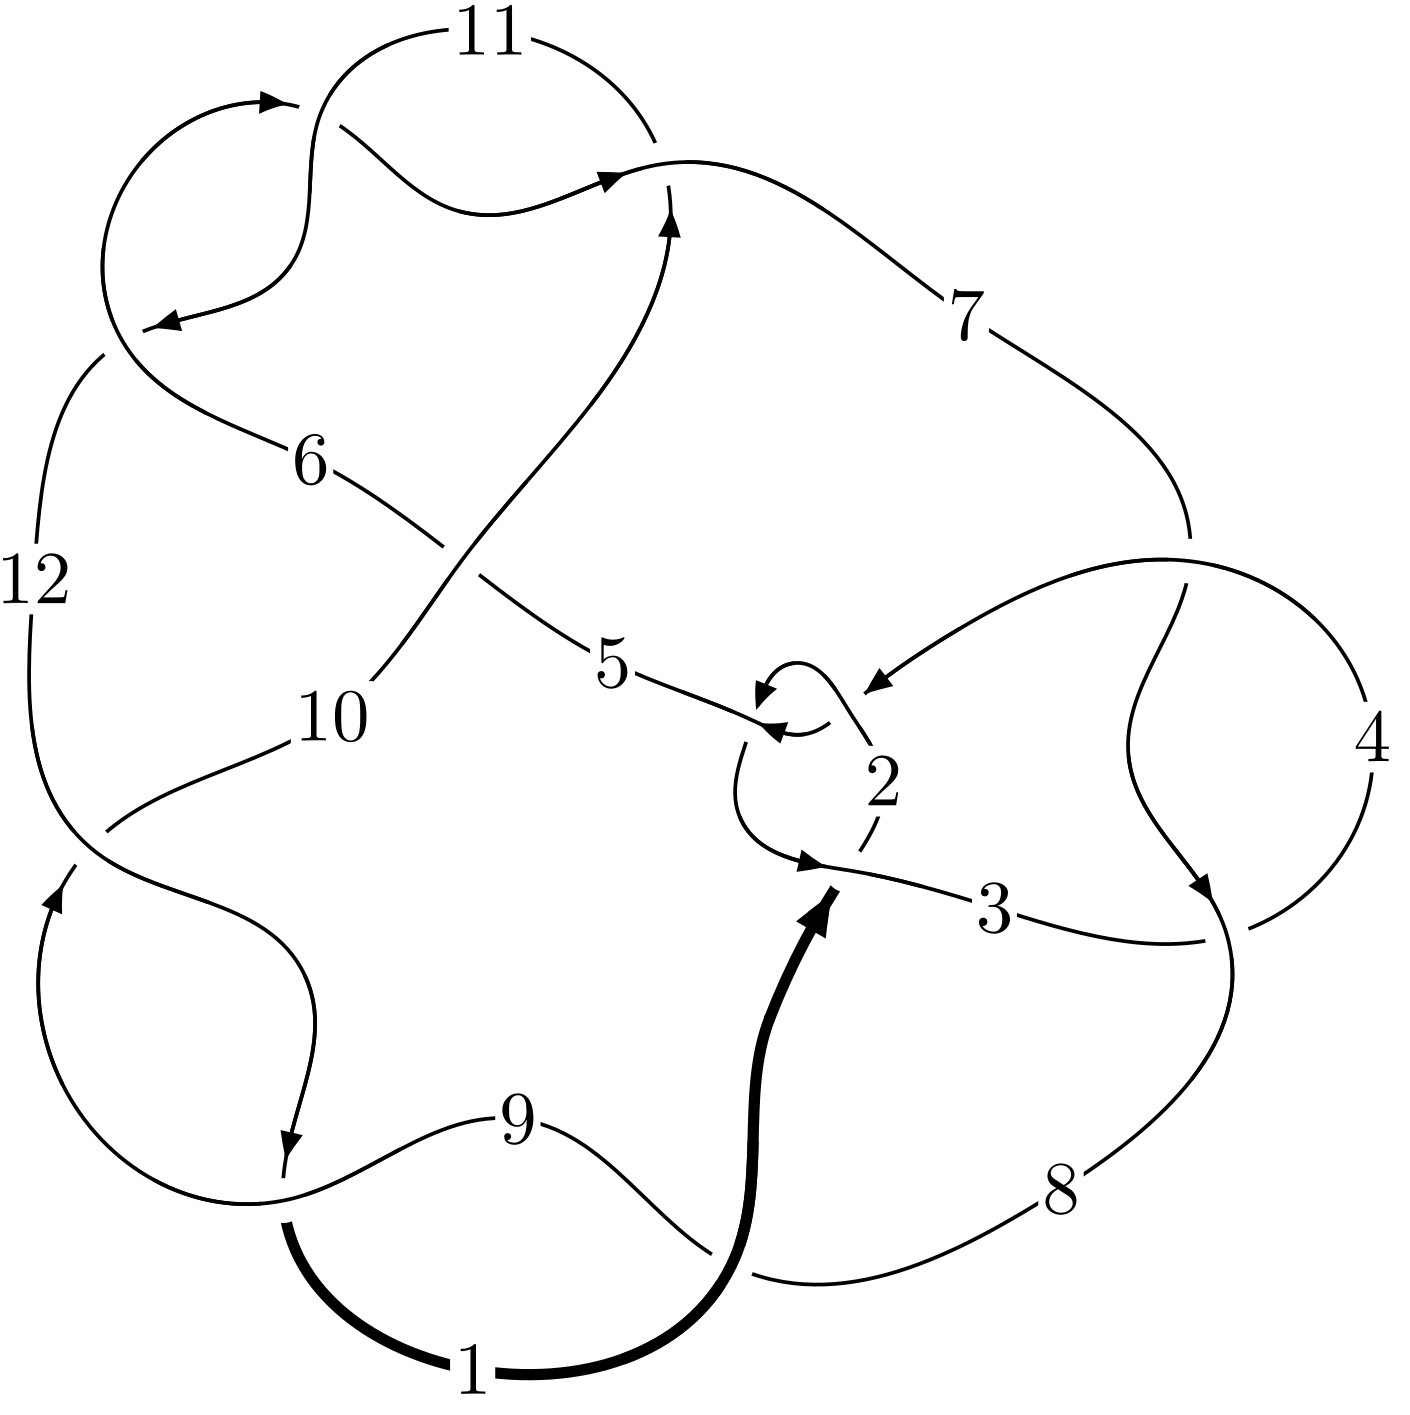
\includegraphics[width=112pt]{../../../GIT/diagram.site/Diagrams/png/898_12a_0097.png}\\
\ \ \ A knot diagram\footnotemark}&
\allowdisplaybreaks
\textbf{Linearized knot diagam} \\
\cline{2-2}
 &
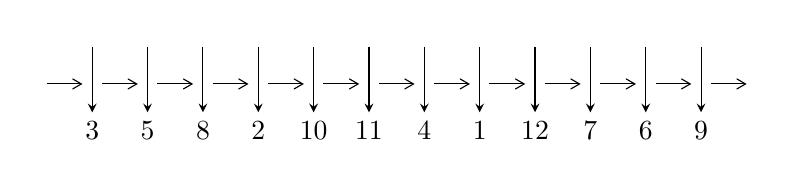
\begin{tikzpicture}[x=20pt, y=17pt]
	% nodes
	\node (C0) at (0, 0) {};
	\node (C1) at (1, 0) {};
	\node (C1U) at (1, +1) {};
	\node (C1D) at (1, -1) {3};

	\node (C2) at (2, 0) {};
	\node (C2U) at (2, +1) {};
	\node (C2D) at (2, -1) {5};

	\node (C3) at (3, 0) {};
	\node (C3U) at (3, +1) {};
	\node (C3D) at (3, -1) {8};

	\node (C4) at (4, 0) {};
	\node (C4U) at (4, +1) {};
	\node (C4D) at (4, -1) {2};

	\node (C5) at (5, 0) {};
	\node (C5U) at (5, +1) {};
	\node (C5D) at (5, -1) {10};

	\node (C6) at (6, 0) {};
	\node (C6U) at (6, +1) {};
	\node (C6D) at (6, -1) {11};

	\node (C7) at (7, 0) {};
	\node (C7U) at (7, +1) {};
	\node (C7D) at (7, -1) {4};

	\node (C8) at (8, 0) {};
	\node (C8U) at (8, +1) {};
	\node (C8D) at (8, -1) {1};

	\node (C9) at (9, 0) {};
	\node (C9U) at (9, +1) {};
	\node (C9D) at (9, -1) {12};

	\node (C10) at (10, 0) {};
	\node (C10U) at (10, +1) {};
	\node (C10D) at (10, -1) {7};

	\node (C11) at (11, 0) {};
	\node (C11U) at (11, +1) {};
	\node (C11D) at (11, -1) {6};

	\node (C12) at (12, 0) {};
	\node (C12U) at (12, +1) {};
	\node (C12D) at (12, -1) {9};
	\node (C13) at (13, 0) {};

	% arrows
	\draw[->,>={angle 60}]
	(C0) edge (C1) (C1) edge (C2) (C2) edge (C3) (C3) edge (C4) (C4) edge (C5) (C5) edge (C6) (C6) edge (C7) (C7) edge (C8) (C8) edge (C9) (C9) edge (C10) (C10) edge (C11) (C11) edge (C12) (C12) edge (C13) ;	\draw[->,>=stealth]
	(C1U) edge (C1D) (C2U) edge (C2D) (C3U) edge (C3D) (C4U) edge (C4D) (C5U) edge (C5D) (C6U) edge (C6D) (C7U) edge (C7D) (C8U) edge (C8D) (C9U) edge (C9D) (C10U) edge (C10D) (C11U) edge (C11D) (C12U) edge (C12D) ;
	\end{tikzpicture} \\
\hhline{~~} \\& 
\textbf{Solving Sequence} \\ \cline{2-2} 
 &
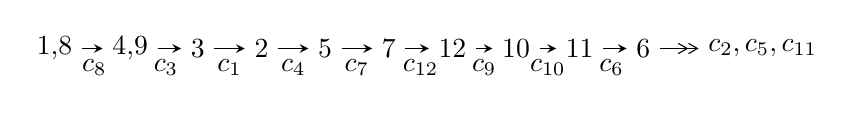
\begin{tikzpicture}[x=23pt, y=7pt]
	% node
	\node (A0) at (-1/8, 0) {1,8};
	\node (A1) at (17/16, 0) {4,9};
	\node (A2) at (17/8, 0) {3};
	\node (A3) at (25/8, 0) {2};
	\node (A4) at (33/8, 0) {5};
	\node (A5) at (41/8, 0) {7};
	\node (A6) at (49/8, 0) {12};
	\node (A7) at (57/8, 0) {10};
	\node (A8) at (65/8, 0) {11};
	\node (A9) at (73/8, 0) {6};
	\node (C1) at (1/2, -1) {$c_{8}$};
	\node (C2) at (13/8, -1) {$c_{3}$};
	\node (C3) at (21/8, -1) {$c_{1}$};
	\node (C4) at (29/8, -1) {$c_{4}$};
	\node (C5) at (37/8, -1) {$c_{7}$};
	\node (C6) at (45/8, -1) {$c_{12}$};
	\node (C7) at (53/8, -1) {$c_{9}$};
	\node (C8) at (61/8, -1) {$c_{10}$};
	\node (C9) at (69/8, -1) {$c_{6}$};
	\node (A10) at (11, 0) {$c_{2},c_{5},c_{11}$};

	% edge
	\draw[->,>=stealth]	
	(A0) edge (A1) (A1) edge (A2) (A2) edge (A3) (A3) edge (A4) (A4) edge (A5) (A5) edge (A6) (A6) edge (A7) (A7) edge (A8) (A8) edge (A9) ;
	\draw[->>,>={angle 60}]	
	(A9) edge (A10);
\end{tikzpicture} \\ 

\end{tabular} \\

\footnotetext{
The image of knot diagram is generated by the software ``\textbf{Draw programme}" developed by Andrew Bartholomew(\url{http://www.layer8.co.uk/maths/draw/index.htm\#Running-draw}), where we modified some parts for our purpose(\url{https://github.com/CATsTAILs/LinksPainter}).
}\phantom \\ \newline 
\centering \textbf{Ideals for irreducible components\footnotemark of $X_{\text{par}}$} 
 
\begin{align*}
I^u_{1}&=\langle 
2.27877\times10^{118} u^{70}-1.71790\times10^{119} u^{69}+\cdots+6.29616\times10^{119} b-2.88028\times10^{119},\\
\phantom{I^u_{1}}&\phantom{= \langle  }-1.11155\times10^{119} u^{70}+7.86535\times10^{119} u^{69}+\cdots+4.40732\times10^{120} a+1.25108\times10^{121},\\
\phantom{I^u_{1}}&\phantom{= \langle  }u^{71}-8 u^{70}+\cdots-336 u+49\rangle \\
I^u_{2}&=\langle 
b,\;u^2+a+2,\;u^3+2 u-1\rangle \\
I^u_{3}&=\langle 
b,\;- u^3- u^2+a-2 u-2,\;u^4+u^3+2 u^2+2 u+1\rangle \\
\\
\end{align*}
\raggedright * 3 irreducible components of $\dim_{\mathbb{C}}=0$, with total 78 representations.\\
\footnotetext{All coefficients of polynomials are rational numbers. But the coefficients are sometimes approximated in decimal forms when there is not enough margin.}
\newpage
\renewcommand{\arraystretch}{1}
\centering \section*{I. $I^u_{1}= \langle 2.28\times10^{118} u^{70}-1.72\times10^{119} u^{69}+\cdots+6.30\times10^{119} b-2.88\times10^{119},\;-1.11\times10^{119} u^{70}+7.87\times10^{119} u^{69}+\cdots+4.41\times10^{120} a+1.25\times10^{121},\;u^{71}-8 u^{70}+\cdots-336 u+49 \rangle$}
\flushleft \textbf{(i) Arc colorings}\\
\begin{tabular}{m{7pt} m{180pt} m{7pt} m{180pt} }
\flushright $a_{1}=$&$\begin{pmatrix}0\\u\end{pmatrix}$ \\
\flushright $a_{8}=$&$\begin{pmatrix}1\\0\end{pmatrix}$ \\
\flushright $a_{4}=$&$\begin{pmatrix}0.0252206 u^{70}-0.178461 u^{69}+\cdots+12.8042 u-2.83865\\-0.0361930 u^{70}+0.272848 u^{69}+\cdots-10.0915 u+0.457467\end{pmatrix}$ \\
\flushright $a_{9}=$&$\begin{pmatrix}1\\u^2\end{pmatrix}$ \\
\flushright $a_{3}=$&$\begin{pmatrix}-0.0109724 u^{70}+0.0943870 u^{69}+\cdots+2.71273 u-2.38119\\-0.0361930 u^{70}+0.272848 u^{69}+\cdots-10.0915 u+0.457467\end{pmatrix}$ \\
\flushright $a_{2}=$&$\begin{pmatrix}-0.0289170 u^{70}+0.232103 u^{69}+\cdots-11.9842 u-0.213372\\-0.00325428 u^{70}+0.0204184 u^{69}+\cdots+4.10649 u-1.07519\end{pmatrix}$ \\
\flushright $a_{5}=$&$\begin{pmatrix}0.0327771 u^{70}-0.219346 u^{69}+\cdots+20.2771 u-2.78303\\-0.00325428 u^{70}+0.0204184 u^{69}+\cdots+4.10649 u-1.07519\end{pmatrix}$ \\
\flushright $a_{7}=$&$\begin{pmatrix}-0.0209275 u^{70}+0.142661 u^{69}+\cdots+14.5291 u-1.66013\\0.0428700 u^{70}-0.321456 u^{69}+\cdots+8.23006 u-1.60608\end{pmatrix}$ \\
\flushright $a_{12}=$&$\begin{pmatrix}u\\u^3+u\end{pmatrix}$ \\
\flushright $a_{10}=$&$\begin{pmatrix}u^2+1\\u^4+2 u^2\end{pmatrix}$ \\
\flushright $a_{11}=$&$\begin{pmatrix}-0.0175926 u^{70}+0.136899 u^{69}+\cdots+12.9847 u-2.05681\\0.0348688 u^{70}-0.279866 u^{69}+\cdots+1.94984 u+0.536966\end{pmatrix}$ \\
\flushright $a_{6}=$&$\begin{pmatrix}0.0410166 u^{70}-0.324779 u^{69}+\cdots+25.3736 u-3.63534\\-0.0478328 u^{70}+0.393772 u^{69}+\cdots-12.0234 u+1.27819\end{pmatrix}$\\&\end{tabular}
\flushleft \textbf{(ii) Obstruction class $= -1$}\\~\\
\flushleft \textbf{(iii) Cusp Shapes $= -0.0549660 u^{70}+0.494164 u^{69}+\cdots-79.5880 u+1.61216$}\\~\\
\newpage\renewcommand{\arraystretch}{1}
\flushleft \textbf{(iv) u-Polynomials at the component}\newline \\
\begin{tabular}{m{50pt}|m{274pt}}
Crossings & \hspace{64pt}u-Polynomials at each crossing \\
\hline $$\begin{aligned}c_{1}\end{aligned}$$&$\begin{aligned}
&u^{71}+30 u^{70}+\cdots+63 u+1
\end{aligned}$\\
\hline $$\begin{aligned}c_{2},c_{4}\end{aligned}$$&$\begin{aligned}
&u^{71}-8 u^{70}+\cdots- u+1
\end{aligned}$\\
\hline $$\begin{aligned}c_{3},c_{7}\end{aligned}$$&$\begin{aligned}
&u^{71}+u^{70}+\cdots+320 u+128
\end{aligned}$\\
\hline $$\begin{aligned}c_{5}\end{aligned}$$&$\begin{aligned}
&u^{71}-2 u^{70}+\cdots-784 u+4360
\end{aligned}$\\
\hline $$\begin{aligned}c_{6},c_{10},c_{11}\end{aligned}$$&$\begin{aligned}
&u^{71}+2 u^{70}+\cdots+4 u+1
\end{aligned}$\\
\hline $$\begin{aligned}c_{8},c_{9},c_{12}\end{aligned}$$&$\begin{aligned}
&u^{71}-8 u^{70}+\cdots-336 u+49
\end{aligned}$\\
\hline
\end{tabular}\\~\\
\newpage\renewcommand{\arraystretch}{1}
\flushleft \textbf{(v) Riley Polynomials at the component}\newline \\
\begin{tabular}{m{50pt}|m{274pt}}
Crossings & \hspace{64pt}Riley Polynomials at each crossing \\
\hline $$\begin{aligned}c_{1}\end{aligned}$$&$\begin{aligned}
&y^{71}+30 y^{70}+\cdots+3271 y-1
\end{aligned}$\\
\hline $$\begin{aligned}c_{2},c_{4}\end{aligned}$$&$\begin{aligned}
&y^{71}-30 y^{70}+\cdots+63 y-1
\end{aligned}$\\
\hline $$\begin{aligned}c_{3},c_{7}\end{aligned}$$&$\begin{aligned}
&y^{71}+45 y^{70}+\cdots-233472 y-16384
\end{aligned}$\\
\hline $$\begin{aligned}c_{5}\end{aligned}$$&$\begin{aligned}
&y^{71}+36 y^{70}+\cdots-370918384 y-19009600
\end{aligned}$\\
\hline $$\begin{aligned}c_{6},c_{10},c_{11}\end{aligned}$$&$\begin{aligned}
&y^{71}+68 y^{70}+\cdots+12 y-1
\end{aligned}$\\
\hline $$\begin{aligned}c_{8},c_{9},c_{12}\end{aligned}$$&$\begin{aligned}
&y^{71}+80 y^{70}+\cdots-77420 y-2401
\end{aligned}$\\
\hline
\end{tabular}\\~\\
\newpage\flushleft \textbf{(vi) Complex Volumes and Cusp Shapes}
$$\begin{array}{c|c|c}  
\text{Solutions to }I^u_{1}& \I (\text{vol} + \sqrt{-1}CS) & \text{Cusp shape}\\
 \hline 
\begin{aligned}
u &= \phantom{-}0.965089 + 0.222646 I \\
a &= -0.463055 + 0.146640 I \\
b &= -0.383523 - 1.048760 I\end{aligned}
 & \phantom{-}2.17116 - 4.96264 I & \phantom{-0.000000 } 0 \\ \hline\begin{aligned}
u &= \phantom{-}0.965089 - 0.222646 I \\
a &= -0.463055 - 0.146640 I \\
b &= -0.383523 + 1.048760 I\end{aligned}
 & \phantom{-}2.17116 + 4.96264 I & \phantom{-0.000000 } 0 \\ \hline\begin{aligned}
u &= \phantom{-}0.555630 + 0.843517 I \\
a &= -0.179841 - 0.287942 I \\
b &= -0.921031 + 0.373991 I\end{aligned}
 & \phantom{-}3.18386 - 5.21037 I & \phantom{-0.000000 } 0 \\ \hline\begin{aligned}
u &= \phantom{-}0.555630 - 0.843517 I \\
a &= -0.179841 + 0.287942 I \\
b &= -0.921031 - 0.373991 I\end{aligned}
 & \phantom{-}3.18386 + 5.21037 I & \phantom{-0.000000 } 0 \\ \hline\begin{aligned}
u &= -0.497939 + 0.886784 I \\
a &= -0.460887 - 0.886344 I \\
b &= -0.213854 + 1.051720 I\end{aligned}
 & \phantom{-}2.29580 + 2.43328 I & \phantom{-0.000000 } 0 \\ \hline\begin{aligned}
u &= -0.497939 - 0.886784 I \\
a &= -0.460887 + 0.886344 I \\
b &= -0.213854 - 1.051720 I\end{aligned}
 & \phantom{-}2.29580 - 2.43328 I & \phantom{-0.000000 } 0 \\ \hline\begin{aligned}
u &= \phantom{-}0.901281 + 0.483012 I \\
a &= \phantom{-}0.174621 - 0.074659 I \\
b &= -0.183485 + 0.929838 I\end{aligned}
 & \phantom{-}2.82109 - 0.79303 I & \phantom{-0.000000 } 0 \\ \hline\begin{aligned}
u &= \phantom{-}0.901281 - 0.483012 I \\
a &= \phantom{-}0.174621 + 0.074659 I \\
b &= -0.183485 - 0.929838 I\end{aligned}
 & \phantom{-}2.82109 + 0.79303 I & \phantom{-0.000000 } 0 \\ \hline\begin{aligned}
u &= -0.737991 + 0.797805 I \\
a &= \phantom{-}0.817472 + 0.829674 I \\
b &= \phantom{-}0.496722 - 1.174470 I\end{aligned}
 & \phantom{-}0.78928 + 7.49831 I & \phantom{-0.000000 } 0 \\ \hline\begin{aligned}
u &= -0.737991 - 0.797805 I \\
a &= \phantom{-}0.817472 - 0.829674 I \\
b &= \phantom{-}0.496722 + 1.174470 I\end{aligned}
 & \phantom{-}0.78928 - 7.49831 I & \phantom{-0.000000 } 0\\
 \hline 
 \end{array}$$\newpage$$\begin{array}{c|c|c}  
\text{Solutions to }I^u_{1}& \I (\text{vol} + \sqrt{-1}CS) & \text{Cusp shape}\\
 \hline 
\begin{aligned}
u &= -0.898468 + 0.151332 I \\
a &= \phantom{-}0.0921622 + 0.0914888 I \\
b &= \phantom{-}0.274475 + 1.005400 I\end{aligned}
 & -1.11803 - 2.10911 I & \phantom{-0.000000 } 0 \\ \hline\begin{aligned}
u &= -0.898468 - 0.151332 I \\
a &= \phantom{-}0.0921622 - 0.0914888 I \\
b &= \phantom{-}0.274475 - 1.005400 I\end{aligned}
 & -1.11803 + 2.10911 I & \phantom{-0.000000 } 0 \\ \hline\begin{aligned}
u &= \phantom{-}0.519063 + 0.701175 I \\
a &= -0.45976 + 2.32557 I \\
b &= -0.267550 - 0.775200 I\end{aligned}
 & \phantom{-}2.27830 - 2.99192 I & \phantom{-0.000000 } 0 \\ \hline\begin{aligned}
u &= \phantom{-}0.519063 - 0.701175 I \\
a &= -0.45976 - 2.32557 I \\
b &= -0.267550 + 0.775200 I\end{aligned}
 & \phantom{-}2.27830 + 2.99192 I & \phantom{-0.000000 } 0 \\ \hline\begin{aligned}
u &= \phantom{-}0.542453 + 1.060010 I \\
a &= \phantom{-}0.312954 - 1.139310 I \\
b &= \phantom{-}0.336812 + 1.112900 I\end{aligned}
 & \phantom{-}7.64845 - 5.36975 I & \phantom{-0.000000 } 0 \\ \hline\begin{aligned}
u &= \phantom{-}0.542453 - 1.060010 I \\
a &= \phantom{-}0.312954 + 1.139310 I \\
b &= \phantom{-}0.336812 - 1.112900 I\end{aligned}
 & \phantom{-}7.64845 + 5.36975 I & \phantom{-0.000000 } 0 \\ \hline\begin{aligned}
u &= -0.170069 + 1.204310 I \\
a &= -0.021614 - 0.362936 I \\
b &= -0.002806 + 0.626003 I\end{aligned}
 & \phantom{-}2.50967 + 1.94105 I & \phantom{-0.000000 } 0 \\ \hline\begin{aligned}
u &= -0.170069 - 1.204310 I \\
a &= -0.021614 + 0.362936 I \\
b &= -0.002806 - 0.626003 I\end{aligned}
 & \phantom{-}2.50967 - 1.94105 I & \phantom{-0.000000 } 0 \\ \hline\begin{aligned}
u &= \phantom{-}0.345350 + 0.682566 I \\
a &= \phantom{-}1.018120 - 0.634027 I \\
b &= \phantom{-}0.044806 + 1.135950 I\end{aligned}
 & \phantom{-}3.18971 + 0.88617 I & -5.37424 - 3.34259 I \\ \hline\begin{aligned}
u &= \phantom{-}0.345350 - 0.682566 I \\
a &= \phantom{-}1.018120 + 0.634027 I \\
b &= \phantom{-}0.044806 - 1.135950 I\end{aligned}
 & \phantom{-}3.18971 - 0.88617 I & -5.37424 + 3.34259 I\\
 \hline 
 \end{array}$$\newpage$$\begin{array}{c|c|c}  
\text{Solutions to }I^u_{1}& \I (\text{vol} + \sqrt{-1}CS) & \text{Cusp shape}\\
 \hline 
\begin{aligned}
u &= -0.478584 + 0.568662 I \\
a &= \phantom{-}0.568000 - 0.216623 I \\
b &= \phantom{-}0.803895 + 0.353915 I\end{aligned}
 & -1.82493 + 2.59268 I & -15.3769 - 7.2742 I \\ \hline\begin{aligned}
u &= -0.478584 - 0.568662 I \\
a &= \phantom{-}0.568000 + 0.216623 I \\
b &= \phantom{-}0.803895 - 0.353915 I\end{aligned}
 & -1.82493 - 2.59268 I & -15.3769 + 7.2742 I \\ \hline\begin{aligned}
u &= \phantom{-}0.738278 + 1.040830 I \\
a &= -0.667814 + 1.062280 I \\
b &= -0.552812 - 1.199040 I\end{aligned}
 & \phantom{-}5.84593 - 10.65120 I & \phantom{-0.000000 } 0 \\ \hline\begin{aligned}
u &= \phantom{-}0.738278 - 1.040830 I \\
a &= -0.667814 - 1.062280 I \\
b &= -0.552812 + 1.199040 I\end{aligned}
 & \phantom{-}5.84593 + 10.65120 I & \phantom{-0.000000 } 0 \\ \hline\begin{aligned}
u &= \phantom{-}0.551600 + 0.463905 I \\
a &= -1.304920 + 0.339654 I \\
b &= -0.394465 - 1.185760 I\end{aligned}
 & \phantom{-}2.25258 - 4.24592 I & -7.24520 + 3.14949 I \\ \hline\begin{aligned}
u &= \phantom{-}0.551600 - 0.463905 I \\
a &= -1.304920 - 0.339654 I \\
b &= -0.394465 + 1.185760 I\end{aligned}
 & \phantom{-}2.25258 + 4.24592 I & -7.24520 - 3.14949 I \\ \hline\begin{aligned}
u &= \phantom{-}0.700493 + 0.073725 I \\
a &= -0.99238 - 1.19225 I \\
b &= -0.604080 + 0.530248 I\end{aligned}
 & \phantom{-}0.487722 - 1.022320 I & -13.68239 - 0.22891 I \\ \hline\begin{aligned}
u &= \phantom{-}0.700493 - 0.073725 I \\
a &= -0.99238 + 1.19225 I \\
b &= -0.604080 - 0.530248 I\end{aligned}
 & \phantom{-}0.487722 + 1.022320 I & -13.68239 + 0.22891 I \\ \hline\begin{aligned}
u &= -0.016841 + 0.702643 I \\
a &= -1.54871 - 1.43918 I \\
b &= -0.040877 + 1.295280 I\end{aligned}
 & \phantom{-}9.32963 - 2.62843 I & -1.88831 + 2.84842 I \\ \hline\begin{aligned}
u &= -0.016841 - 0.702643 I \\
a &= -1.54871 + 1.43918 I \\
b &= -0.040877 - 1.295280 I\end{aligned}
 & \phantom{-}9.32963 + 2.62843 I & -1.88831 - 2.84842 I\\
 \hline 
 \end{array}$$\newpage$$\begin{array}{c|c|c}  
\text{Solutions to }I^u_{1}& \I (\text{vol} + \sqrt{-1}CS) & \text{Cusp shape}\\
 \hline 
\begin{aligned}
u &= \phantom{-}0.332568 + 0.605833 I \\
a &= -0.301092 + 0.636346 I \\
b &= \phantom{-}0.862872 - 0.007307 I\end{aligned}
 & \phantom{-}4.21028 - 1.36691 I & -5.92252 + 0.19732 I \\ \hline\begin{aligned}
u &= \phantom{-}0.332568 - 0.605833 I \\
a &= -0.301092 - 0.636346 I \\
b &= \phantom{-}0.862872 + 0.007307 I\end{aligned}
 & \phantom{-}4.21028 + 1.36691 I & -5.92252 - 0.19732 I \\ \hline\begin{aligned}
u &= \phantom{-}0.558598 + 0.272901 I \\
a &= -0.299568 - 0.501299 I \\
b &= \phantom{-}0.440934 + 0.406344 I\end{aligned}
 & \phantom{-}3.36702 - 1.57403 I & -6.09432 + 4.24770 I \\ \hline\begin{aligned}
u &= \phantom{-}0.558598 - 0.272901 I \\
a &= -0.299568 + 0.501299 I \\
b &= \phantom{-}0.440934 - 0.406344 I\end{aligned}
 & \phantom{-}3.36702 + 1.57403 I & -6.09432 - 4.24770 I \\ \hline\begin{aligned}
u &= -0.435436 + 0.347884 I \\
a &= \phantom{-}1.09728 + 2.39333 I \\
b &= \phantom{-}0.316131 - 0.580635 I\end{aligned}
 & -2.50844 + 0.67754 I & -14.4694 - 9.3694 I \\ \hline\begin{aligned}
u &= -0.435436 - 0.347884 I \\
a &= \phantom{-}1.09728 - 2.39333 I \\
b &= \phantom{-}0.316131 + 0.580635 I\end{aligned}
 & -2.50844 - 0.67754 I & -14.4694 + 9.3694 I \\ \hline\begin{aligned}
u &= \phantom{-}0.27752 + 1.42324 I \\
a &= \phantom{-}0.031422 - 0.333514 I \\
b &= -0.015427 + 0.624053 I\end{aligned}
 & \phantom{-}8.54375 - 5.00674 I & \phantom{-0.000000 } 0 \\ \hline\begin{aligned}
u &= \phantom{-}0.27752 - 1.42324 I \\
a &= \phantom{-}0.031422 + 0.333514 I \\
b &= -0.015427 - 0.624053 I\end{aligned}
 & \phantom{-}8.54375 + 5.00674 I & \phantom{-0.000000 } 0 \\ \hline\begin{aligned}
u &= -0.097939 + 0.485793 I \\
a &= \phantom{-}2.58622 + 1.57725 I \\
b &= \phantom{-}0.361070 - 1.308120 I\end{aligned}
 & \phantom{-}8.54074 + 3.06263 I & -3.03957 - 2.89556 I \\ \hline\begin{aligned}
u &= -0.097939 - 0.485793 I \\
a &= \phantom{-}2.58622 - 1.57725 I \\
b &= \phantom{-}0.361070 + 1.308120 I\end{aligned}
 & \phantom{-}8.54074 - 3.06263 I & -3.03957 + 2.89556 I\\
 \hline 
 \end{array}$$\newpage$$\begin{array}{c|c|c}  
\text{Solutions to }I^u_{1}& \I (\text{vol} + \sqrt{-1}CS) & \text{Cusp shape}\\
 \hline 
\begin{aligned}
u &= -0.06886 + 1.50531 I \\
a &= \phantom{-}0.01135 + 2.28493 I \\
b &= \phantom{-}0.024006 - 1.065750 I\end{aligned}
 & \phantom{-}3.67289 + 2.17680 I & \phantom{-0.000000 } 0 \\ \hline\begin{aligned}
u &= -0.06886 - 1.50531 I \\
a &= \phantom{-}0.01135 - 2.28493 I \\
b &= \phantom{-}0.024006 + 1.065750 I\end{aligned}
 & \phantom{-}3.67289 - 2.17680 I & \phantom{-0.000000 } 0 \\ \hline\begin{aligned}
u &= \phantom{-}0.00316 + 1.51912 I \\
a &= \phantom{-}0.444013 - 0.011181 I \\
b &= -1.166440 + 0.191892 I\end{aligned}
 & \phantom{-}5.33599 - 0.33795 I & \phantom{-0.000000 } 0 \\ \hline\begin{aligned}
u &= \phantom{-}0.00316 - 1.51912 I \\
a &= \phantom{-}0.444013 + 0.011181 I \\
b &= -1.166440 - 0.191892 I\end{aligned}
 & \phantom{-}5.33599 + 0.33795 I & \phantom{-0.000000 } 0 \\ \hline\begin{aligned}
u &= -0.12329 + 1.54920 I \\
a &= -0.430159 - 0.078037 I \\
b &= \phantom{-}1.170270 + 0.230752 I\end{aligned}
 & \phantom{-}5.25008 + 4.73327 I & \phantom{-0.000000 } 0 \\ \hline\begin{aligned}
u &= -0.12329 - 1.54920 I \\
a &= -0.430159 + 0.078037 I \\
b &= \phantom{-}1.170270 - 0.230752 I\end{aligned}
 & \phantom{-}5.25008 - 4.73327 I & \phantom{-0.000000 } 0 \\ \hline\begin{aligned}
u &= \phantom{-}0.15624 + 1.55244 I \\
a &= -0.48688 + 1.73940 I \\
b &= -0.61601 - 1.36943 I\end{aligned}
 & \phantom{-}9.10594 - 6.74702 I & \phantom{-0.000000 } 0 \\ \hline\begin{aligned}
u &= \phantom{-}0.15624 - 1.55244 I \\
a &= -0.48688 - 1.73940 I \\
b &= -0.61601 + 1.36943 I\end{aligned}
 & \phantom{-}9.10594 + 6.74702 I & \phantom{-0.000000 } 0 \\ \hline\begin{aligned}
u &= -0.04061 + 1.56679 I \\
a &= \phantom{-}0.47782 + 1.82859 I \\
b &= \phantom{-}0.61104 - 1.39480 I\end{aligned}
 & \phantom{-}15.6993 + 3.6198 I & \phantom{-0.000000 } 0 \\ \hline\begin{aligned}
u &= -0.04061 - 1.56679 I \\
a &= \phantom{-}0.47782 - 1.82859 I \\
b &= \phantom{-}0.61104 + 1.39480 I\end{aligned}
 & \phantom{-}15.6993 - 3.6198 I & \phantom{-0.000000 } 0\\
 \hline 
 \end{array}$$\newpage$$\begin{array}{c|c|c}  
\text{Solutions to }I^u_{1}& \I (\text{vol} + \sqrt{-1}CS) & \text{Cusp shape}\\
 \hline 
\begin{aligned}
u &= \phantom{-}0.08851 + 1.58806 I \\
a &= -0.499554 + 0.013294 I \\
b &= \phantom{-}1.192900 + 0.167411 I\end{aligned}
 & \phantom{-}11.75780 - 2.86927 I & \phantom{-0.000000 } 0 \\ \hline\begin{aligned}
u &= \phantom{-}0.08851 - 1.58806 I \\
a &= -0.499554 - 0.013294 I \\
b &= \phantom{-}1.192900 - 0.167411 I\end{aligned}
 & \phantom{-}11.75780 + 2.86927 I & \phantom{-0.000000 } 0 \\ \hline\begin{aligned}
u &= \phantom{-}0.07767 + 1.59080 I \\
a &= \phantom{-}0.31543 - 1.81519 I \\
b &= \phantom{-}0.36546 + 1.43425 I\end{aligned}
 & \phantom{-}10.92660 - 0.53406 I & \phantom{-0.000000 } 0 \\ \hline\begin{aligned}
u &= \phantom{-}0.07767 - 1.59080 I \\
a &= \phantom{-}0.31543 + 1.81519 I \\
b &= \phantom{-}0.36546 - 1.43425 I\end{aligned}
 & \phantom{-}10.92660 + 0.53406 I & \phantom{-0.000000 } 0 \\ \hline\begin{aligned}
u &= \phantom{-}0.14393 + 1.59724 I \\
a &= -0.01779 + 2.26870 I \\
b &= -0.048367 - 1.098220 I\end{aligned}
 & \phantom{-}10.02040 - 5.42403 I & \phantom{-0.000000 } 0 \\ \hline\begin{aligned}
u &= \phantom{-}0.14393 - 1.59724 I \\
a &= -0.01779 - 2.26870 I \\
b &= -0.048367 + 1.098220 I\end{aligned}
 & \phantom{-}10.02040 + 5.42403 I & \phantom{-0.000000 } 0 \\ \hline\begin{aligned}
u &= \phantom{-}0.00999 + 1.62086 I \\
a &= -0.32346 - 1.87968 I \\
b &= -0.35353 + 1.46380 I\end{aligned}
 & \phantom{-}17.4703 - 2.6861 I & \phantom{-0.000000 } 0 \\ \hline\begin{aligned}
u &= \phantom{-}0.00999 - 1.62086 I \\
a &= -0.32346 + 1.87968 I \\
b &= -0.35353 - 1.46380 I\end{aligned}
 & \phantom{-}17.4703 + 2.6861 I & \phantom{-0.000000 } 0 \\ \hline\begin{aligned}
u &= -0.15869 + 1.63585 I \\
a &= -0.25913 - 1.78272 I \\
b &= -0.39647 + 1.42419 I\end{aligned}
 & \phantom{-}10.77460 + 5.03788 I & \phantom{-0.000000 } 0 \\ \hline\begin{aligned}
u &= -0.15869 - 1.63585 I \\
a &= -0.25913 + 1.78272 I \\
b &= -0.39647 - 1.42419 I\end{aligned}
 & \phantom{-}10.77460 - 5.03788 I & \phantom{-0.000000 } 0\\
 \hline 
 \end{array}$$\newpage$$\begin{array}{c|c|c}  
\text{Solutions to }I^u_{1}& \I (\text{vol} + \sqrt{-1}CS) & \text{Cusp shape}\\
 \hline 
\begin{aligned}
u &= -0.23701 + 1.62979 I \\
a &= \phantom{-}0.42275 + 1.68597 I \\
b &= \phantom{-}0.63809 - 1.35812 I\end{aligned}
 & \phantom{-}8.8506 + 11.2317 I & \phantom{-0.000000 } 0 \\ \hline\begin{aligned}
u &= -0.23701 - 1.62979 I \\
a &= \phantom{-}0.42275 - 1.68597 I \\
b &= \phantom{-}0.63809 + 1.35812 I\end{aligned}
 & \phantom{-}8.8506 - 11.2317 I & \phantom{-0.000000 } 0 \\ \hline\begin{aligned}
u &= \phantom{-}0.17330 + 1.64014 I \\
a &= \phantom{-}0.465694 - 0.121420 I \\
b &= -1.196240 + 0.249549 I\end{aligned}
 & \phantom{-}11.58050 - 8.05691 I & \phantom{-0.000000 } 0 \\ \hline\begin{aligned}
u &= \phantom{-}0.17330 - 1.64014 I \\
a &= \phantom{-}0.465694 + 0.121420 I \\
b &= -1.196240 - 0.249549 I\end{aligned}
 & \phantom{-}11.58050 + 8.05691 I & \phantom{-0.000000 } 0 \\ \hline\begin{aligned}
u &= -0.313436\phantom{ +0.000000I} \\
a &= \phantom{-}0.420211\phantom{ +0.000000I} \\
b &= -0.362858\phantom{ +0.000000I}\end{aligned}
 & -0.621610\phantom{ +0.000000I} & -15.9200\phantom{ +0.000000I} \\ \hline\begin{aligned}
u &= \phantom{-}0.050078 + 0.277688 I \\
a &= -0.89153 + 1.57529 I \\
b &= -0.664853 + 0.126557 I\end{aligned}
 & -0.930568 - 0.261352 I & -10.83012 - 1.62800 I \\ \hline\begin{aligned}
u &= \phantom{-}0.050078 - 0.277688 I \\
a &= -0.89153 - 1.57529 I \\
b &= -0.664853 - 0.126557 I\end{aligned}
 & -0.930568 + 0.261352 I & -10.83012 + 1.62800 I \\ \hline\begin{aligned}
u &= \phantom{-}0.18363 + 1.71053 I \\
a &= \phantom{-}0.20893 - 1.79674 I \\
b &= \phantom{-}0.42095 + 1.43650 I\end{aligned}
 & \phantom{-}17.1323 - 8.4610 I & \phantom{-0.000000 } 0 \\ \hline\begin{aligned}
u &= \phantom{-}0.18363 - 1.71053 I \\
a &= \phantom{-}0.20893 + 1.79674 I \\
b &= \phantom{-}0.42095 - 1.43650 I\end{aligned}
 & \phantom{-}17.1323 + 8.4610 I & \phantom{-0.000000 } 0 \\ \hline\begin{aligned}
u &= \phantom{-}0.24399 + 1.71973 I \\
a &= -0.36048 + 1.69027 I \\
b &= -0.65719 - 1.36333 I\end{aligned}
 & \phantom{-}15.1368 - 14.7023 I & \phantom{-0.000000 } 0\\
 \hline 
 \end{array}$$\newpage$$\begin{array}{c|c|c}  
\text{Solutions to }I^u_{1}& \I (\text{vol} + \sqrt{-1}CS) & \text{Cusp shape}\\
 \hline 
\begin{aligned}
u &= \phantom{-}0.24399 - 1.71973 I \\
a &= -0.36048 - 1.69027 I \\
b &= -0.65719 + 1.36333 I\end{aligned}
 & \phantom{-}15.1368 + 14.7023 I & \phantom{-0.000000 } 0\\
 \hline 
 \end{array}$$\newpage\newpage\renewcommand{\arraystretch}{1}
\centering \section*{II. $I^u_{2}= \langle b,\;u^2+a+2,\;u^3+2 u-1 \rangle$}
\flushleft \textbf{(i) Arc colorings}\\
\begin{tabular}{m{7pt} m{180pt} m{7pt} m{180pt} }
\flushright $a_{1}=$&$\begin{pmatrix}0\\u\end{pmatrix}$ \\
\flushright $a_{8}=$&$\begin{pmatrix}1\\0\end{pmatrix}$ \\
\flushright $a_{4}=$&$\begin{pmatrix}- u^2-2\\0\end{pmatrix}$ \\
\flushright $a_{9}=$&$\begin{pmatrix}1\\u^2\end{pmatrix}$ \\
\flushright $a_{3}=$&$\begin{pmatrix}- u^2-2\\0\end{pmatrix}$ \\
\flushright $a_{2}=$&$\begin{pmatrix}- u^2-2\\u\end{pmatrix}$ \\
\flushright $a_{5}=$&$\begin{pmatrix}0\\- u\end{pmatrix}$ \\
\flushright $a_{7}=$&$\begin{pmatrix}1\\0\end{pmatrix}$ \\
\flushright $a_{12}=$&$\begin{pmatrix}u\\- u+1\end{pmatrix}$ \\
\flushright $a_{10}=$&$\begin{pmatrix}u^2+1\\u\end{pmatrix}$ \\
\flushright $a_{11}=$&$\begin{pmatrix}u^2- u+1\\u\end{pmatrix}$ \\
\flushright $a_{6}=$&$\begin{pmatrix}u^2+u\\- u^2\end{pmatrix}$\\&\end{tabular}
\flushleft \textbf{(ii) Obstruction class $= 1$}\\~\\
\flushleft \textbf{(iii) Cusp Shapes $= - u^2-3 u-14$}\\~\\
\newpage\renewcommand{\arraystretch}{1}
\flushleft \textbf{(iv) u-Polynomials at the component}\newline \\
\begin{tabular}{m{50pt}|m{274pt}}
Crossings & \hspace{64pt}u-Polynomials at each crossing \\
\hline $$\begin{aligned}c_{1},c_{2}\end{aligned}$$&$\begin{aligned}
&(u-1)^3
\end{aligned}$\\
\hline $$\begin{aligned}c_{3},c_{7}\end{aligned}$$&$\begin{aligned}
&u^3
\end{aligned}$\\
\hline $$\begin{aligned}c_{4}\end{aligned}$$&$\begin{aligned}
&(u+1)^3
\end{aligned}$\\
\hline $$\begin{aligned}c_{5}\end{aligned}$$&$\begin{aligned}
&u^3-3 u^2+5 u-2
\end{aligned}$\\
\hline $$\begin{aligned}c_{6},c_{8},c_{9}\end{aligned}$$&$\begin{aligned}
&u^3+2 u-1
\end{aligned}$\\
\hline $$\begin{aligned}c_{10},c_{11},c_{12}\end{aligned}$$&$\begin{aligned}
&u^3+2 u+1
\end{aligned}$\\
\hline
\end{tabular}\\~\\
\newpage\renewcommand{\arraystretch}{1}
\flushleft \textbf{(v) Riley Polynomials at the component}\newline \\
\begin{tabular}{m{50pt}|m{274pt}}
Crossings & \hspace{64pt}Riley Polynomials at each crossing \\
\hline $$\begin{aligned}c_{1},c_{2},c_{4}\end{aligned}$$&$\begin{aligned}
&(y-1)^3
\end{aligned}$\\
\hline $$\begin{aligned}c_{3},c_{7}\end{aligned}$$&$\begin{aligned}
&y^3
\end{aligned}$\\
\hline $$\begin{aligned}c_{5}\end{aligned}$$&$\begin{aligned}
&y^3+y^2+13 y-4
\end{aligned}$\\
\hline $$\begin{aligned}c_{6},c_{8},c_{9}\\c_{10},c_{11},c_{12}\end{aligned}$$&$\begin{aligned}
&y^3+4 y^2+4 y-1
\end{aligned}$\\
\hline
\end{tabular}\\~\\
\newpage\flushleft \textbf{(vi) Complex Volumes and Cusp Shapes}
$$\begin{array}{c|c|c}  
\text{Solutions to }I^u_{2}& \I (\text{vol} + \sqrt{-1}CS) & \text{Cusp shape}\\
 \hline 
\begin{aligned}
u &= -0.22670 + 1.46771 I \\
a &= \phantom{-}0.102785 + 0.665457 I \\
b &= \phantom{-0.000000 } 0\end{aligned}
 & \phantom{-}7.79580 + 5.13794 I & -11.21712 - 3.73768 I \\ \hline\begin{aligned}
u &= -0.22670 - 1.46771 I \\
a &= \phantom{-}0.102785 - 0.665457 I \\
b &= \phantom{-0.000000 } 0\end{aligned}
 & \phantom{-}7.79580 - 5.13794 I & -11.21712 + 3.73768 I \\ \hline\begin{aligned}
u &= \phantom{-}0.453398\phantom{ +0.000000I} \\
a &= -2.20557\phantom{ +0.000000I} \\
b &= \phantom{-0.000000 } 0\end{aligned}
 & -2.43213\phantom{ +0.000000I} & -15.5660\phantom{ +0.000000I}\\
 \hline 
 \end{array}$$\newpage\newpage\renewcommand{\arraystretch}{1}
\centering \section*{III. $I^u_{3}= \langle b,\;- u^3- u^2+a-2 u-2,\;u^4+u^3+2 u^2+2 u+1 \rangle$}
\flushleft \textbf{(i) Arc colorings}\\
\begin{tabular}{m{7pt} m{180pt} m{7pt} m{180pt} }
\flushright $a_{1}=$&$\begin{pmatrix}0\\u\end{pmatrix}$ \\
\flushright $a_{8}=$&$\begin{pmatrix}1\\0\end{pmatrix}$ \\
\flushright $a_{4}=$&$\begin{pmatrix}u^3+u^2+2 u+2\\0\end{pmatrix}$ \\
\flushright $a_{9}=$&$\begin{pmatrix}1\\u^2\end{pmatrix}$ \\
\flushright $a_{3}=$&$\begin{pmatrix}u^3+u^2+2 u+2\\0\end{pmatrix}$ \\
\flushright $a_{2}=$&$\begin{pmatrix}u^3+u^2+2 u+2\\u\end{pmatrix}$ \\
\flushright $a_{5}=$&$\begin{pmatrix}0\\- u\end{pmatrix}$ \\
\flushright $a_{7}=$&$\begin{pmatrix}1\\0\end{pmatrix}$ \\
\flushright $a_{12}=$&$\begin{pmatrix}u\\u^3+u\end{pmatrix}$ \\
\flushright $a_{10}=$&$\begin{pmatrix}u^2+1\\- u^3-2 u-1\end{pmatrix}$ \\
\flushright $a_{11}=$&$\begin{pmatrix}u^3+u^2+2 u+2\\- u^3-2 u-1\end{pmatrix}$ \\
\flushright $a_{6}=$&$\begin{pmatrix}u^3+2 u+1\\u^3+u^2+u+2\end{pmatrix}$\\&\end{tabular}
\flushleft \textbf{(ii) Obstruction class $= 1$}\\~\\
\flushleft \textbf{(iii) Cusp Shapes $= -2 u^3+2 u^2- u-12$}\\~\\
\newpage\renewcommand{\arraystretch}{1}
\flushleft \textbf{(iv) u-Polynomials at the component}\newline \\
\begin{tabular}{m{50pt}|m{274pt}}
Crossings & \hspace{64pt}u-Polynomials at each crossing \\
\hline $$\begin{aligned}c_{1},c_{2}\end{aligned}$$&$\begin{aligned}
&(u-1)^4
\end{aligned}$\\
\hline $$\begin{aligned}c_{3},c_{7}\end{aligned}$$&$\begin{aligned}
&u^4
\end{aligned}$\\
\hline $$\begin{aligned}c_{4}\end{aligned}$$&$\begin{aligned}
&(u+1)^4
\end{aligned}$\\
\hline $$\begin{aligned}c_{5}\end{aligned}$$&$\begin{aligned}
&(u^2+u+1)^2
\end{aligned}$\\
\hline $$\begin{aligned}c_{6},c_{8},c_{9}\end{aligned}$$&$\begin{aligned}
&u^4+u^3+2 u^2+2 u+1
\end{aligned}$\\
\hline $$\begin{aligned}c_{10},c_{11},c_{12}\end{aligned}$$&$\begin{aligned}
&u^4- u^3+2 u^2-2 u+1
\end{aligned}$\\
\hline
\end{tabular}\\~\\
\newpage\renewcommand{\arraystretch}{1}
\flushleft \textbf{(v) Riley Polynomials at the component}\newline \\
\begin{tabular}{m{50pt}|m{274pt}}
Crossings & \hspace{64pt}Riley Polynomials at each crossing \\
\hline $$\begin{aligned}c_{1},c_{2},c_{4}\end{aligned}$$&$\begin{aligned}
&(y-1)^4
\end{aligned}$\\
\hline $$\begin{aligned}c_{3},c_{7}\end{aligned}$$&$\begin{aligned}
&y^4
\end{aligned}$\\
\hline $$\begin{aligned}c_{5}\end{aligned}$$&$\begin{aligned}
&(y^2+y+1)^2
\end{aligned}$\\
\hline $$\begin{aligned}c_{6},c_{8},c_{9}\\c_{10},c_{11},c_{12}\end{aligned}$$&$\begin{aligned}
&y^4+3 y^3+2 y^2+1
\end{aligned}$\\
\hline
\end{tabular}\\~\\
\newpage\flushleft \textbf{(vi) Complex Volumes and Cusp Shapes}
$$\begin{array}{c|c|c}  
\text{Solutions to }I^u_{3}& \I (\text{vol} + \sqrt{-1}CS) & \text{Cusp shape}\\
 \hline 
\begin{aligned}
u &= -0.621744 + 0.440597 I \\
a &= \phantom{-}1.070700 + 0.758745 I \\
b &= \phantom{-0.000000 } 0\end{aligned}
 & \phantom{-}1.64493 + 2.02988 I & -11.23686 - 2.38721 I \\ \hline\begin{aligned}
u &= -0.621744 - 0.440597 I \\
a &= \phantom{-}1.070700 - 0.758745 I \\
b &= \phantom{-0.000000 } 0\end{aligned}
 & \phantom{-}1.64493 - 2.02988 I & -11.23686 + 2.38721 I \\ \hline\begin{aligned}
u &= \phantom{-}0.121744 + 1.306620 I \\
a &= -0.070696 + 0.758745 I \\
b &= \phantom{-0.000000 } 0\end{aligned}
 & \phantom{-}1.64493 - 2.02988 I & -14.2631 + 3.6750 I \\ \hline\begin{aligned}
u &= \phantom{-}0.121744 - 1.306620 I \\
a &= -0.070696 - 0.758745 I \\
b &= \phantom{-0.000000 } 0\end{aligned}
 & \phantom{-}1.64493 + 2.02988 I & -14.2631 - 3.6750 I\\
 \hline 
 \end{array}$$\newpage
\newpage\renewcommand{\arraystretch}{1}
\centering \section*{ IV. u-Polynomials}
\begin{tabular}{m{50pt}|m{274pt}}
Crossings & \hspace{64pt}u-Polynomials at each crossing \\
\hline $$\begin{aligned}c_{1}\end{aligned}$$&$\begin{aligned}
&((u-1)^7)(u^{71}+30 u^{70}+\cdots+63 u+1)
\end{aligned}$\\
\hline $$\begin{aligned}c_{2}\end{aligned}$$&$\begin{aligned}
&((u-1)^7)(u^{71}-8 u^{70}+\cdots- u+1)
\end{aligned}$\\
\hline $$\begin{aligned}c_{3},c_{7}\end{aligned}$$&$\begin{aligned}
&u^7(u^{71}+u^{70}+\cdots+320 u+128)
\end{aligned}$\\
\hline $$\begin{aligned}c_{4}\end{aligned}$$&$\begin{aligned}
&((u+1)^7)(u^{71}-8 u^{70}+\cdots- u+1)
\end{aligned}$\\
\hline $$\begin{aligned}c_{5}\end{aligned}$$&$\begin{aligned}
&((u^2+u+1)^2)(u^3-3 u^2+5 u-2)(u^{71}-2 u^{70}+\cdots-784 u+4360)
\end{aligned}$\\
\hline $$\begin{aligned}c_{6}\end{aligned}$$&$\begin{aligned}
&(u^3+2 u-1)(u^4+u^3+2 u^2+2 u+1)(u^{71}+2 u^{70}+\cdots+4 u+1)
\end{aligned}$\\
\hline $$\begin{aligned}c_{8},c_{9}\end{aligned}$$&$\begin{aligned}
&(u^3+2 u-1)(u^4+u^3+2 u^2+2 u+1)(u^{71}-8 u^{70}+\cdots-336 u+49)
\end{aligned}$\\
\hline $$\begin{aligned}c_{10},c_{11}\end{aligned}$$&$\begin{aligned}
&(u^3+2 u+1)(u^4- u^3+2 u^2-2 u+1)(u^{71}+2 u^{70}+\cdots+4 u+1)
\end{aligned}$\\
\hline $$\begin{aligned}c_{12}\end{aligned}$$&$\begin{aligned}
&(u^3+2 u+1)(u^4- u^3+2 u^2-2 u+1)(u^{71}-8 u^{70}+\cdots-336 u+49)
\end{aligned}$\\
\hline
\end{tabular}\newpage\renewcommand{\arraystretch}{1}
\centering \section*{ V. Riley Polynomials}
\begin{tabular}{m{50pt}|m{274pt}}
Crossings & \hspace{64pt}Riley Polynomials at each crossing \\
\hline $$\begin{aligned}c_{1}\end{aligned}$$&$\begin{aligned}
&((y-1)^7)(y^{71}+30 y^{70}+\cdots+3271 y-1)
\end{aligned}$\\
\hline $$\begin{aligned}c_{2},c_{4}\end{aligned}$$&$\begin{aligned}
&((y-1)^7)(y^{71}-30 y^{70}+\cdots+63 y-1)
\end{aligned}$\\
\hline $$\begin{aligned}c_{3},c_{7}\end{aligned}$$&$\begin{aligned}
&y^7(y^{71}+45 y^{70}+\cdots-233472 y-16384)
\end{aligned}$\\
\hline $$\begin{aligned}c_{5}\end{aligned}$$&$\begin{aligned}
&(y^2+y+1)^2(y^3+y^2+13 y-4)\\
&\cdot(y^{71}+36 y^{70}+\cdots-370918384 y-19009600)
\end{aligned}$\\
\hline $$\begin{aligned}c_{6},c_{10},c_{11}\end{aligned}$$&$\begin{aligned}
&(y^3+4 y^2+4 y-1)(y^4+3 y^3+2 y^2+1)(y^{71}+68 y^{70}+\cdots+12 y-1)
\end{aligned}$\\
\hline $$\begin{aligned}c_{8},c_{9},c_{12}\end{aligned}$$&$\begin{aligned}
&(y^3+4 y^2+4 y-1)(y^4+3 y^3+2 y^2+1)\\
&\cdot(y^{71}+80 y^{70}+\cdots-77420 y-2401)
\end{aligned}$\\
\hline
\end{tabular}
\vskip 2pc
\end{document}